\section{Den bagvedlæggende kemi}
Stort set alle kemiske forbindelser, der indeholder kovalente bindinger absorberer nogle specielle frekvenser af elektromagnetisk stråling i den infrarøde del af det elektromagnetiske spektrum.\refSpektroskopi{13} Det interval vi beskæftiger os med når vi ser på IR-spektroskopi ligger i intervallet $2,5 \mu m- 25 \mu m $. Det er de bølgelængder af det infrarøde lys, som giver den vibrationelle effekt på atomerne og molekylerne som vi søger. Når vi i afsnit \ref{IRSPEK} skal se på 3 forskellige IR-spektre, vil der hen af x-aksen være plottet reciprokke centimeter. Dette skyldes, at kemikere af konvention laver bølgelængder om til \textbf{bølgetal}, \={v} , ved at tage den reciprokke værdi af bølgelængden i cm.\refSpektroskopi{13}

\begin{center}
\={v}$= \dfrac{1}{\lambda}$
\end{center}

Den primære grund til at bølgetal foretrækkes over bølgelængde er, at bølgetallene er direkte proportionelle til energien af de fotoner, som lyset består af. På den måde vil et højere bølgetal repræsenterer en højere energi. Bølgetal kan laves om til en frekvens ved at gange det med lysets hastighed, c, for så at puttes ind i formlen for fotonenergi $E_{fot} = h \cdot f$, hvor h er plancks konstant og f er frekvens i $\frac{1}{s}$. 
\\

Det ses at fotonenergien bliver større ved et større bølgetal 
\\

\begin{center}
$f =$ \={v} $\cdot c \rightarrow$ \={v} $\cdot c \cdot h = E_{fot}$
\end{center}

Som med alle former for stråling vil molekyler der rammes blive exciteret til et højere energiniveau ved absorbtion af den infrarøde stråling. Det resultat der gør IR-spektroskopi interessant er, at  forskellige molekyler svinger med forskellige frekvenser og derfor optager forskellige bølgelængder af lys. De frekvenser som molekylerne absorberer svarer lige præcist til de egenfrekvenser som molekylerne får når atomerne, der er bundet sammen af kovalente bindinger, enten bøjer eller svinger som vist på figur \ref{fig:spek}. 
\\

Siden alle bånd har en forskellig egenfrekvenser, da de befinder sig i lidt forskellige $miljøer$, vil to molekyler give forskellige udslag på et infrarødt spektrum.\refSpektroskopi{15} Selvom nogle absorbtionsmønstre kan være de samme - hvis begge molekyler eksempelvis indeholder en fælles funktionel gruppe - vil de to molekyler stadigvæk give nogle udslag som adskiller sig fra hinanden, medmindre at stofferne selvfølgelig er identiske. IR-spektre for kemiske forbindelser kan på den måde betragtes den kemiske pendant til menneskets fingeraftryk. Dette betyder at bindinger mellem atomer vil give udslag i små intervaller, der er kendetegnende for netop disse bindinger. Eksempelvis vil et udslag i området $2150cm^{-1}$ formegentligt være 2 carbonatomer, der er tribbeltbundet til hinanden og 2 carbonatomer der er dobbeltbundet til hinanden vil blive fundet området omkring $1650cm^{-1}$. Vi kan slå disse værdier op i en databog
\\

Atomerne i molekylerne der er bundet sammen af kovalente bånd kan svinge på forskellige måder. De simpleste vibrationelle bevægelser i molekyler, som er $infrarøde$ $aktive$ er bindinger som strækker sig eller bøjer.
\\

Der er andre, mere komplicerede måder, som bindingerne mellem atomerne i molekylerne kan opføre sig på. De kan også $sakse$ (scissoring), $rokke$ (rocking), $twiste$ (twisting) og $rykke$ (wagging). 
\\

\begin{center}
\begin{figure}
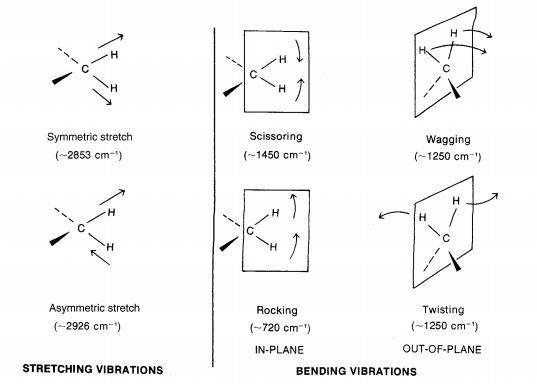
\includegraphics[scale=1]{Billeder/streak}
\caption{Illustration af forskellige vibrationer: Billedet er fra s. 16 i "Introduction to Spectroscopy" \label{fig:spek}}
\end{figure}
\end{center}

Lad os nu se på hvordan vi kan beregne bølgetal for bestemte atom- og funktionelle grupper. Hvis vi nu ser på et af de simpleste eksempler for vibrationer mellem atomer; et diatomisk molekyle med en strækkende vibration. Her kan vi betragte den kovalente binding mellem de to atomer som en fjeder. Et diatomisk molekyle kan betragtes som en fjeder hvor båndlængden bliver ved med at ændre sig. Dette betyder nødvendigvis at den kovalente binding, eller fjederen, må have en frekvens som den vibrerer med. Det gælder at energien for en harmonisk oscillerende bevægelse mellem atomer er direkte proportionelt med frekvensen for den harmoniske oscillator givet ved formlen

\begin{center}
\begin{equation}
E_{osc} \propto h f_{osc}
\end{equation}
\end{center}

For et diatomisk molekyle er det, der bestemmer frekvensen i den harmonisk oscillerende bevægelse størrelserne, k (fjederkonstanten) og masserne af de to atomer der indgår i bindingen $m_1$ og $m_2$.
\\

Frekvensen for en harmonisk oscillerende vibration mellem to atomer er givet ved formlen:

\begin{center}
\={v}$= \dfrac{1}{2 \pi c} \sqrt[2]{\dfrac{k}{\mu}}$
\end{center}

Denne formel er udledt fra Hookes lov for vibrerende fjedre.\refSpektroskopi{18} her er k, fjederkonstanten, \={v} er bølgetallet og $\mu$ er den reducerede masse givet ved formlen $\mu = \frac{m_1 m_2}{m_1 + m_2}$. 
\\

Da det ikke altid er lige praktisk at bruge massen af atomer til at finde bølgetallet, kan man i stedet omskrive lidt på formlen således at der kan regnes på molarmassen af de to atomer i stedet for deres masse.
\\

I stedet for $\mu = \dfrac{m_1 m_2}{m_1 + m_2}$ kan vi skrive $\mu = \dfrac{m_1 m_2}{m_1 + m_2} = \dfrac{M_1 M_2}{(M_1 + M_2 ) (6.02 \cdot 10^{23})}$. 
\\

Vi kan altså udtrykket masserne som molarmasser ved at dividere $\mu$ udtrykt ved masse, med Avogadros tal $N_A$.
\\

Avogadros tal flyttes ud foran kvadratrodstegnet ved at tage kvadratroden af det og putte det i tælleren på den første brøk således at der står:

\begin{center}
\={v}$(cm^{-1})=\dfrac{\sqrt[2]{6.02 \cdot 10^{23}}}{2 \pi c} \cdot \sqrt[2]{\dfrac{K}{\mu}} = \dfrac{7.76 \cdot 10^{11}}{2 \pi c} \cdot \sqrt[2]{\dfrac{K}{\mu}}$
\end{center}

Her er $\mu$ ikke massen længere, men \emph{molarmassen}.
\\

Udtrykket kan reduceres yderligere ved at udregne værdien af den  første brøk, så vi får formlen

\begin{center}
\={v}$=4.12 \sqrt[2]{\dfrac{K}{\mu}}$
\end{center}

Hvor $\mu$ er den reduerede molarmasse og k er fjederkonstanten for systemet i \emph{dynes} per. centimeter. Dynes er mål for kraft. $10^5$  $dynes = 1N$.
\\

Som en approksimation bruger vi respektivt K = 5, 10, 15 $\cdot 10^5 \frac{dynes}{cm}$ for enkelt, dobbelt og trippeltbindinger.
\\

For at validere denne formel vil vi se på 2 eksempler hvor bølgetallet er bestemt gennem et eksperiment sammenligne det med de værdier der opnås når formlen bruges. Vi betragter først dobbeltbindingen mellem carbonatomerne i ethen.
\\

Det bølgetal, der er bestemt ved forsøg er \={v}$=1650cm^{-1}$\refSpektroskopi{21}. Hvis vi bruger formlen til at regne bølgetallet ud får vi: $4.12 \cdot \sqrt[2]{\dfrac{10 \cdot 10^5}{(\frac{12 \cdot 12}{12 +12})}} = 1682 cm^{-1}$. 
\\

Et andet eksempel er bindingen mellem et carbonatom og et hydrogenatom. Her er der tale om en enkeltbinding og vi bruger da $K=5 \cdot 10^5 \frac{dynes}{cm}$ og en $\mu = \frac{12 \cdot 1}{12 + 1} = 0.9231$. Putter vi det ind i formlen får vi et bølgetal på: $4.12 \cdot \sqrt[2]{\dfrac{5 \cdot 10^5}{0.9231}} \approx 3032 cm^{-1}$. Bølgetallet for stræk mellem C og H er ved forsøg bestemt til at være 3000.\refSpektroskopi{21} 
\\

Formlen giver os altså et godt bud på hvor vi kan forvente at se bølgetal for stræk mellem to atomer.
\\

Vi vil lige diskutere betydningen af k samt hvad der har indflydelse på størrelsen af k. 
\subsection{Fjederkonstanten for bindingen mellem diatomiske molekyler}

I normale fjedre vil fjederkonstanten, som navnet antyder, være konstant lige gyldigt hvad vi hænger i den. Dette gør sig egentligt også gældende for de kovalente bindinger mellem molekyler, hvis de vel at mærke er underlagt præcist de samme betingelser. 
\\

Et større k medfører et større bølgetal, da tælleren bliver større og værdien for $\sqrt[2]{\dfrac{K}{\mu}}$ da bliver større. Det er derfor vigtigt, at se på de faktorer der bestemmer værdien af k.
\\

\textbf{Betydninger for værdien af k}
\begin{enumerate}
\item Det gælder som en regel at værdien af fjederkonstanten, k, er tre gange så høj for tripeltbindinger som for enkeltbindinger og at k er dobbelt så høj for dobbeltbindinger som for enkeltbindinger. Vi sætter disse værdier af k til at være henholdsvis 5, 10 og 15 for enkelt-, dobbelt- og trippeltbindinger. Vi vil senere diskutere i hvor stor grad denne tommelfingerregel for beregninger af bølgetal holder.

\item Hybdridisering har også en effekt på værdien af k. Som regel er bånd stærkere i rækkefølgen $sp > sp^2 > sp^3$. Dette kan vi se hvis vi betragter enkeltbundne, dobbeltbundne og trippeltbundne carbonatomer, der også binder sig til et hydrogenatom:

\begin{center}
\begin{figure}

\includegraphics[scale=1]{Billeder/sp}
\caption{Billedet er fra s. 19 i "Introduction to Spectroscopy"}
\end{figure}
\end{center}


\end{enumerate}

For det andet vil store atomer der er bundet til atomer, der er relativt mindre end dem selv vibrerer ved højere frekvenser, da værdien af $\mu$ vil være mindre og gøre $\sqrt[2]{\dfrac{K}{\mu}}$ større. 
\\

Vi kan tjekke om dette passer ved at slå op i en databog og se på bølgetal for forskellige atomer bundet sammen:
\\
\begin{figure}
\includegraphics[scale=1]{Billeder/udklip}
\caption{Billedet er taget fra s. 18 i "Introduction to Spectroscopy"}
\end{figure}

Billedet viser, at jo større et atom carbon er bundet til jo større bliver $\mu$ og derfor også bølgetallet \={v}.

Bevægelser mellem atomer, der er bøjende vil også optræde ved en lavere energi, og altså også ved et lavere \={v}, end de strækkende bevægelser. Eksempelvis vil C-H stræk give udslag ved et bølgetal på ca. 3000 $cm^{-1}$ mens C-H bøj vil give et udsalg omkring $1340cm^{-1}$.

\subsubsection{Hookes lov som model for interaktion mellem atomer}
I forrige afsnit fandt vi frem til formlen:

\begin{center}
\={v}$=4.12 \sqrt[2]{\dfrac{K}{\mu}}$
\end{center}

Denne formel utrolig brugbar til at regne bølgetal ud for vibrationer mellem to atomer. Vi skal dog notere os, at formlen kun kan bruges til at regne bølgetallet ud for strækkende vibrationer mellem to atomer, da formlen er udledt ud fra Hookes lov, som beskriver en fjeder som bliver enten trukket i eller presset sammen. Formlen beskriver altså ikke de andre former for \emph{vibrationer} som buk, saks og tvist.
\\

Derudover bruger vi i den selv samme formel følgende værdier for k: $5 \cdot 10^5 dynes$ for enkeltbindinger, $10 \cdot 10^5 dynes$ for dobbeltbindinger og $15 \cdot 10^5 dynes$ for trippeltbindinger. Vi viste, at disse værdier passede godt for de to eksempler med methan og ethen, men hvis vi husker hvad vi fandt ud af i \ref{sec:del} ville fjederkonstanten for et system være lig summen af alle de fjederkonstanter, som var med i systemet.
\\

Antag at fjeder-/kraftkonstanterne for henholdsvis enkelt-, dobbelt- og tripeltbininger er $5 \cdot, 10 \cdot$ og $15 \cdot 10^5 dynes$. Der vil nu føres et argument for at disse værdier af k leder til en absurditet. 
\\
\textbf{Da enhederne i følgende argument er de samme undlades de i regnestykket af simplicitet}
\\
Hvis vi ser på et system med en dobbeltbinding skal fjeder-/kraftkonstanten være 10. Da en dobbeltbinding også indeholder en $\sigma$-binding kan vi tillade os jævnførende resultatet i \ref{sec:del} at trække fjederkonstanten for en $\sigma$-binding fra, som er 5. Dette efterlader os med en fjederkonstant på 5 som vi skal tildele til de resterende fjedre i systemet. Da vi kun har en $\pi$-binding tilbage må vi enten have at $\pi$-bindingen er lige så stærk som $\sigma$-bindingen, hvilket er falskt. Eller, hvis vi regner $\pi$-bindingen som 2 svage fjedre over for hinanden på hver sin side af $\sigma$-bindingen, at $\sigma$-bindinger er præcist dobbelt så stærke som $\pi$-bindinger - hvilket også er falskt.
\\

Derfor er antagelsen om at enkelt-, dobbelt- og trippeltbindinger respektivt kan gives værdierne $5 \cdot, 10 \cdot$ og $15 \cdot 10^5 dynes$ for k en antagelse og ikke et udtryk for værdiens virkelighed. 